\subsubsection{Activity Diagram - Module Công tác Xã hội}

    Để minh họa chi tiết luồng xử lý của các chức năng chính trong module Công tác Xã hội, báo cáo trình bày 3 Activity Diagram đại diện cho các pattern quan trọng trong hệ thống:
    
    \begin{itemize}
        \item \textbf{Quản lý trạng thái:} Tạo và chỉnh sửa hoạt động với logic chuyển đổi giữa trạng thái Nháp và Đang hoạt động (UC7.3)
        \item \textbf{Xử lý hàng loạt:} Chấm điểm sinh viên từ file Excel với pipeline parse - validate - preview - batch update (UC7.2)
        \item \textbf{Cấu hình cascade:} Tạo cấu hình giới hạn tự động áp dụng cho tổ chức con theo cấp bậc (UC7.4)
    \end{itemize}

    Mỗi diagram thể hiện luồng xử lý hoàn chỉnh từ đầu vào của người dùng đến kết quả cuối cùng, bao gồm các điểm phân nhánh (decision point) và xử lý ngoại lệ quan trọng.

    % ========================================
    % Activity Diagram UC7.3 - Tạo/Chỉnh sửa hoạt động
    \newpage
    \begin{figure}[H]
        \centering
        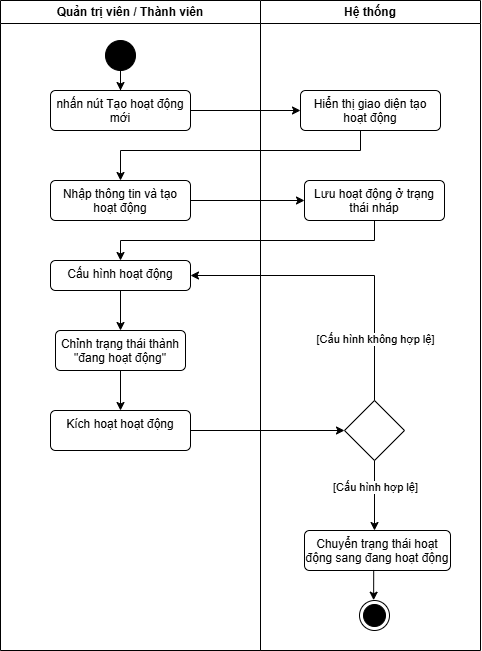
\includegraphics[width=0.75\linewidth]{Images/activity-diagram/UC07_03_tao_chinh_sua_hoat_dong.png}
        \vspace{0.3em}
        \captionsetup{skip=8pt}
        \caption{Activity Diagram - Tạo và chỉnh sửa hoạt động}
        \label{fig:activity-uc07-03}
    \end{figure}

    Activity Diagram trên minh họa luồng tạo và chỉnh sửa hoạt động CTXH với logic quản lý trạng thái. Điểm quan trọng: khi chọn trạng thái "Đang hoạt động", hệ thống yêu cầu validate đầy đủ thông tin (địa điểm, thời gian, số ngày), trong khi trạng thái "Nháp" cho phép lưu không đầy đủ để tiếp tục sau. Hệ thống kiểm tra cấu hình giới hạn số ngày theo tổ chức nhưng chỉ hiển thị cảnh báo, vẫn cho phép tạo hoạt động vượt giới hạn để linh hoạt với các trường hợp đặc biệt.

    % ========================================
    % Activity Diagram UC7.2 - Chấm điểm Excel
    \newpage
    \begin{figure}[H]
        \centering
        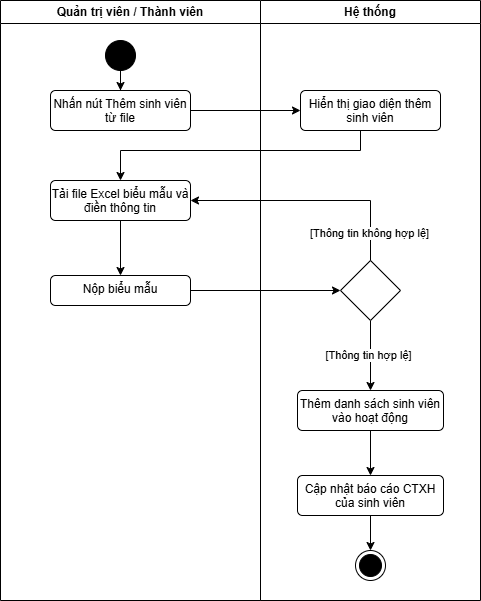
\includegraphics[width=0.75\linewidth]{Images/activity-diagram/UC07_02_cham_diem_excel.png}
        \vspace{0.3em}
        \captionsetup{skip=8pt}
        \caption{Activity Diagram - Chấm điểm sinh viên từ file Excel}
        \label{fig:activity-uc07-02}
    \end{figure}

    Activity Diagram thể hiện luồng xử lý hàng loạt điểm CTXH từ file Excel theo pipeline: parse file $\rightarrow$ validate từng row $\rightarrow$ preview kết quả $\rightarrow$ batch update. Hệ thống xử lý chunk 500 rows để tối ưu hiệu năng với file lớn, validate từng row theo các quy tắc nghiệp vụ (số ngày là bội 0.5, không vượt giới hạn hoạt động, sinh viên tồn tại và đã đăng ký). Trong màn hình preview, các row lỗi được đánh dấu rõ ràng với lý do cụ thể, chỉ các row hợp lệ được cập nhật vào database. Nếu có lỗi trong quá trình batch update, toàn bộ transaction sẽ được rollback để đảm bảo tính nhất quán dữ liệu.

    % ========================================
    % Activity Diagram UC7.4 - Tạo cấu hình giới hạn
    \newpage
    \begin{figure}[H]
        \centering
        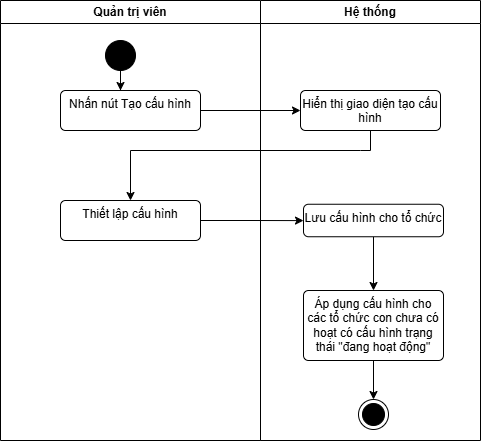
\includegraphics[width=0.75\linewidth]{Images/activity-diagram/UC07_04_tao_cau_hinh_gioi_han.png}
        \vspace{0.3em}
        \captionsetup{skip=8pt}
        \caption{Activity Diagram - Tạo cấu hình giới hạn ngày CTXH}
        \label{fig:activity-uc07-04}
    \end{figure}

    Activity Diagram minh họa luồng tạo cấu hình giới hạn số ngày CTXH với cơ chế cascade tự động. Sau khi tạo cấu hình cho tổ chức cha, hệ thống tự động duyệt qua tất cả tổ chức con cấp 1 và cấp 2 theo cấu trúc phân cấp. Với mỗi tổ chức con, hệ thống kiểm tra: nếu chưa có cấu hình thì tạo mới, nếu đã có cấu hình đang hoạt động thì cập nhật số ngày tối đa. Logic này đảm bảo cấu hình được áp dụng nhất quán cho toàn bộ cây tổ chức mà không cần quản trị viên phải thiết lập thủ công từng tổ chức con.
